% !TeX root = ../main.tex

\chapter{Dirac Band Theory}

\section{Introduction to Graphene}

\paragraph{Why $\mu$ in graphene is very high}
\begin{enumext}
  \item Dirac band: $m^* = 0$.
  \item Electron-phonon scattering is weak.
  \item $\tau_i$ increase: $\mu_i$ increase.
\end{enumext}

\subsection{Honeycomb lattice and its Brillouin zone}

Two vectors
\[
  a_1 = \frac a2(1,\sqrt3), \quad
  a_2 = \frac a2(1,-\sqrt3)
\]
\begin{paracol}{2}
We want to get the $E(k)$ relation, so we obtain the reciprocal lattice first
\[
  b_1 = \frac{2\pi}{a}\ab(1, \frac{\sqrt3}{3}),\quad
  b_2 = \frac{2\pi}{a}\ab(-1, \frac{\sqrt3}{3}).
\]
with the first Brillouin zone
\[
  k = \frac{4\pi}{3a}(1,0), \quad k' = \frac{4\pi}{3a}(-1,0).
\]
\switchcolumn \centering
  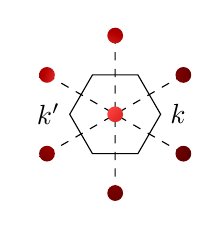
\begin{tikzpicture}
    \draw
      (0:{1/sqrt(3)}) node [right] {$k$} --  (60:{1/sqrt(3)}) --
      (120:{1/sqrt(3)}) -- (180:{1/sqrt(3)}) node [left] {$k'$} --
      (240:{1/sqrt(3)}) -- (300:{1/sqrt(3)}) -- cycle;
    \draw [dashed]
      (150:1) -- (150:-1)
      (90:1) -- (90:-1)
      (30:1) -- (30:-1);
    \shade [ball color = red]
      (0,0) circle (.1)
      (30:1) circle (.1)
      (90:1) circle (.1)
      (150:1) circle (.1)
      (210:1) circle (.1)
      (270:1) circle (.1)
      (330:1) circle (.1);
  \end{tikzpicture}
\end{paracol}

\subsection{Tight-binding method to calculate band structure of graphene}

The Boloch wave function
\begin{align}
  \psi_A & = \frac1{\sqrt N} \sum_{\bm R_A}^N \upe^{\iu\bm k \cdot \bm R_A}
    \varphi_A(\bm r - \bm R_A),\\
  \psi_B & = \frac1{\sqrt N} \sum_{\bm R_B}^N \upe^{\iu\bm k \cdot \bm R_A}
    \varphi_B(\bm r - \bm R_B)
\end{align}
where $\psi_A$ denotes the atomic orbital of A-atom, also for $\psi_B$.
The total wavefunction
\begin{equation}
  \psi = \sum_n b_n\psi_n = b_A \psi_A + b_B \psi_b
= b_A \frac1{\sqrt N} \sum_{R_A} \upe^{\iu\bm k \cdot\bm R_A}
  \varphi_A(\bm r - \bm R_A) +
  b_B \frac1{\sqrt N} \sum_{R_B} \upe^{\iu\bm k \cdot\bm R_B}
  \varphi_B(\bm r - \bm R_B)
\end{equation}
The eigen function
\[
  \hat H\ket|\psi> = E\ket|\psi>
\]
Project all the wavefunction of A-atom
\[
  \braket<\psi_A|\hat H|\psi> = E\braket<\psi_A|\psi>
\]
Then, we have
\begin{multline}
  b_A \frac1{\sqrt N} \sum_{R_A} \upe^{\iu\bm k \cdot\bm R_A}
  \braket<\varphi_A|\hat H|\varphi_{A'}(\bm r - \bm R_A)> +
  b_B \frac1{\sqrt N} \sum_{R_B} \upe^{\iu\bm k \cdot \bm R_B}
  \braket<\varphi_A|\hat H|\varphi_B(\bm r - \bm R_B)>\\
= E\ab[b_A\frac1{\sqrt N} \sum_{R_A}\upe^{\iu\bm k\cdot \bm R_A}
    \braket<\varphi_A|\varphi_A(\bm r - \bm R_A)> +
    b_B \frac1{\sqrt N} \sum_{R_A} \upe^{\iu\bm k\cdot\bm R_B}
    \braket<\varphi_A|\varphi_B(\bm r - \bm R_B)>]
\end{multline}
Rearrange it
\[
  b_A\braket<\varphi_A|\hat H|\varphi_B> \upe^{\iu\bm k\cdot \bm R_A}
+ b_B\braket<\varphi_A|\hat H||\varphi_B> \sum_{R_B}\upe^{\iu\bm k\cdot \bm R_B}
= E b_A \upe^{\iu\bm k\cdot\bm R_A}
\]
Substitute the orthonormality
$\braket<\varphi_A|\varphi_B> = \delta_{A,B}\epsilon_{A,B}$
\[
  b_A\epsilon_0 + b_Bt\sum_{i = 1,2,3} \upe^{\iu k\cdot k_i} = Eb_A
\]
Finally, we arrive at
\begin{equation}
  b_A\epsilon_0 + b_Bt\sum_i \upe^{\iu k\cdot \delta_i} = E b_a,
\end{equation}
Similarly, we can project by $\bra<\varphi_B|$
\begin{equation}
  b_At\sum_i \upe^{-\iu \bm k\cdot \bm \delta_i} + b_B\epsilon = E b_B
\end{equation}
we define
\[
  f(k) = \sum_i \upe^{\iu\bm k \cdot \bm \delta_i}
\]
Then, we can write them into matrix,
\begin{equation}
  \begin{pmatrix}
    \epsilon_0 & tf(k)\\
    tf^*(k) & \epsilon
  \end{pmatrix}
  \begin{pmatrix}
    b_A\\b_B
  \end{pmatrix} = E
  \begin{pmatrix}
    b_A\\b_B
  \end{pmatrix}, \mathbf A\bm b = E\bm b
\end{equation}
The determine $\det(\mathbf A - \lambda\identity)$ should be zero
\[
  \begin{vmatrix}
    \epsilon_0 - E & tf(k)\\
    tf^*(k) & \epsilon_0 - E
  \end{vmatrix} = 0
\]
We can obtain the $E(k)$ relation
\begin{equation}
  E = \epsilon_0 \pm t|f(k)|.
\end{equation}
Make the replacement
\[
  \bm K = \frac{4\pi}{3a}(1,0) \to (0,0), \quad \bm q = \bm k - \bm K, \quad
  \bm p = \hbar\bm q
\]
Then
\begin{align}
  f(k) & = \upe^{\iu\bm k_xa/\sqrt3}
       + 2\upe^{\iu-\iu k_xa/2\sqrt3}\cos(k_xa/2)
= \upe^{\iu q_ya/\sqrt3} + 2\upe^{\iu q_ya/2\sqrt3},\\
  f(q) & = \cos\ab[\frac{(q_x + \frac{4\pi}{3a})a}{2}]
= \upe^{\iu q_ya/\sqrt3} + 2\upe^{-\iu q_ya/2\sqrt3}
  \ab(\cos\frac{q_xa}{2} \cos\frac{4\pi}{3} - \sin\frac{q_xa}{2} \sin\frac{4\pi}{3})
\end{align}
Expand $f(q)$ to the first order
\begin{equation}
  f(q) = \frac{\sqrt3a}{2} (\iu q_y - q_x) + \iu \frac{a^x}{4} q_x \cdot q_y
= \frac{\sqrt3a}{2}(\iu q_y - q_x)
\end{equation}
We can rewrite
\[
  E(k) = \pm t|f(k)| = \pm t\frac{\sqrt3a}{2\hbar} |q|\hbar = v_F |\bm p|
\]
One can rewrite the Hamiltonian interms of Pauli matrices
\begin{equation}
  H_k(p) = v_F(\sigma_x p_x + \sigma_y p_y) = v_F \bm \sigma \cdot \bm p
\end{equation}

\section{Calculation about TBC}

Using the approximation
\begin{enumext}
  \item Only consider the nearest neighbor hopping
  \[
    \braket<\phi_A|H|\phi_B> \neq 0
  \]
  \[
    \epsilon_0 = 0, \quad E_\pm = \pm V_0|f(\bm k)|
  \]
  \item $f(\bm k) \approx \frac{\sqrt3}{2} a(\iu q_y - \xi q_x)$.
\end{enumext}

\section{Chirality}

\begin{enumext}
  \item For conduction band electron: $\bm\sigma \cdot \bm n = 1$.
  \item For valence band electron: $\bm\sigma \cdot \bm n = -1$.
\end{enumext}

\section{Dirac equation with a mass}

The Hamiltonian
\[
  H_k =
  \begin{pmatrix}
    \Delta & -\gamma_0f(\bm k)\\
    -\gamma_0f^*(\bm k) & -\Delta
  \end{pmatrix}
\]
The energy
\[
  E_\pm = \pm\sqrt{\Delta^2 + (\gamma_0|f(\bm k)|)^2}
= \pm \sqrt{(m_Dv_F^2)^2 + (\hbar v_Fk)^2}
\]
where $m_D = \Delta/v_F^2$.
The gap is
\[
  \Delta E = E_+ - E_-
= 2\sqrt{\Delta^2 + (\gamma_0|f(\bm k)|)^2},
\]
and we can open a gap in the band.

\section{Density of states in Graphene}

\[
  g(E) = g_sg_vvv \frac{|E|}{2\pi\hbar^2v_F^2}
\]
The total carrier density
\[
  n = \int_0^\infty g(E) f(E) \d E
= \int_0^{E_f} \frac{g_sg_N E}{2\pi\hbar^2v_F^2} \d E
= \frac{g_sg_VE}{2\pi\hbar^2v_F^2}\d E
= \frac{g_sg_V}{2\pi\hbar^2v_F^2} \frac12 E_F^2
= \frac{E_f^2}{\pi\hbar^2v_F^2}
\]
where $E_F = \pm\hbar v_F\sqrt{|n|\pi} = \pm\hbar v_Fk_F$.

\section{Massless Dirac fermions}

\[
  m^* = \frac1\hbar/\pdv[2]Ek
\]
For $E = \hbar v_F k$, $\pdv Ek = \hbar v_F$, and $\pdv[2]Ek = 0$,
the effective mass will diverge.
So, for massless particle, $m_0 = 0$, $E = c|p|$.

\section{Bilayer Graphene}

The matrix formations of Schr\"odinger equation
\begin{equation}
  \begin{pmatrix}
    H_{AA} & H_{AB}\\
    H_{BA} & H_{BB}
  \end{pmatrix}\psi =
  \begin{pmatrix}
    \braket<\phi_A|\phi_A> & \braket<\phi_A|\phi_B>\\
    \braket<\phi_B|\phi_A> & \braket<\phi_B|\phi_B>\\
  \end{pmatrix}\psi
\end{equation}
For the nearest hopping, the vectors are defined: $\bm\delta_1$, $\bm\delta_2$,
$\bm \delta_3$ with $\braket<\phi_A|H|\phi_B> \neq 0$.
\begin{paracol}{2}
There are two ways for stacking: $A-A$ stacking and $A-B$ stacking.
The former one is unstable, so we consider the latter one only.

Denote the hopping parameter between $A_i$ and $B_i$ is $\gamma_0$, so
\[
  \gamma_0 = \braket<\phi_{A_1}|H|\phi_{B_1}>
= \braket<\phi_{A_2}|H|\phi_{B_2}>
\]
\switchcolumn \centering
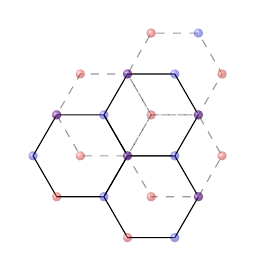
\begin{tikzpicture}[scale = .6]
  \foreach \i in {0,120,240}
    \draw [rotate around = {\i:(0,0)}]
          (0,0) --++ (0:1) --++ (-60:1) --++ (-120:1) --++
          (-180:1) --++ (-240:1) --++ (60:1);
  \begin{scope}[opacity = .4]
  \foreach \i in {0,120,240}
    {
      \shade [rotate around = {\i:(0,0)}, ball color = red]
        (0,{sqrt(3)}) circle (.1);
      \shade [rotate around = {\i:(0,0)}, ball color = red]
        (1.5,{sqrt(3)/2}) circle (.1);
      \shade [rotate around = {\i:(0,0)}, ball color = blue]
        (1,0) circle (.1);
      \shade [rotate around = {\i:(0,0)}, ball color = blue]
        (1,{-sqrt(3)}) circle (.1);
    }
  \shade [ball color = red] (0,0) circle (.1);
  \end{scope}
  \begin{scope}[opacity = .4, shift = {(60:1)}]
  \foreach \i in {0,120,240}
    \draw [dashed, rotate around = {\i:(0,0)}]
          (0,0) --++ (0:1) --++ (-60:1) --++ (-120:1) --++
          (-180:1) --++ (-240:1) --++ (60:1);
  \foreach \i in {0,120,240}
    {
      \shade [rotate around = {\i:(0,0)}, ball color = red]
        (0,{sqrt(3)}) circle (.1);
      \shade [rotate around = {\i:(0,0)}, ball color = red]
        (1.5,{sqrt(3)/2}) circle (.1);
      \shade [rotate around = {\i:(0,0)}, ball color = blue]
        (1,0) circle (.1);
      \shade [rotate around = {\i:(0,0)}, ball color = blue]
        (1,{-sqrt(3)}) circle (.1);
    }
  \shade [ball color = red] (0,0) circle (.1);
  \end{scope}
\end{tikzpicture}\hfill
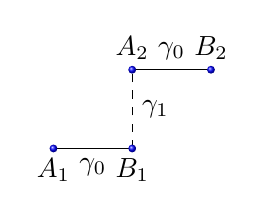
\begin{tikzpicture}
  \draw (-1,0) -- node [below] {$\gamma_0$} (0,0) (0,1) --
   node [above] {$\gamma_0$} (1,1);
  \draw [dashed] (0,0) -- node [right] {$\gamma_1$} (0,1);
  \shade [ball color = blue] (-1,0) circle (.05) node [below] {$A_1$};
  \shade [ball color = blue] (0,0) circle (.05) node [below] {$B_1$};
  \shade [ball color = blue] (0,1) circle (.05) node [above] {$A_2$};
  \shade [ball color = blue] (1,1) circle (.05) node [above] {$B_2$};
\end{tikzpicture}
\end{paracol}
also consider the hopping between $A_i$ and $B_j$, another nearest hopping
the hopping between $A_i$ and $A_j$ can be ignored.
We can write the Sch\"odinger with a labeled Hamiltonian matrix,
the crossing elemets correspoondings to the hopping between the labels.
\[
  \begin{pNiceMatrix}[first-row, last-col]
    A_1 & B_1 & A_2 & B_2\\
    \epsilon_0 - E & -\gamma_0 f(k) & 0 & 0 & A_1\\
    -\gamma_0 f^*(k) & \epsilon_0 - E & \gamma_1 & 0 & B_1\\
    0 & \gamma_1 & \epsilon_0 - E & -\gamma_0 f(k) & A_2\\
    0 & 0 & -\gamma_0 f^*(k) & \epsilon_0 - E & B_1
  \end{pNiceMatrix}\, \bm\psi = 0
\]
where $\epsilon_0$ is a constant value: the site energy;
and $f(k) = \sum_{i=1}^3 \upe^{-\iu k \cdot \delta_k}$.
We can obtain two energies
\begin{equation}
  E_\pm^\alpha = \pm\frac{\gamma_1}{2} \ab(
    \sqrt{1 + \frac{4\gamma_0^2|f(k)|^2}{\gamma_1^2}} + \alpha)
\end{equation}
where $\alpha = \pm 1$.
\begin{enumext}
  \item $\alpha = +1$: $k$, $k'$ valley, $f(k) = 0$,
  \begin{equation}
    E_\pm^{+1} = \pm \frac{\gamma_1}{2} \times 2 = \pm \gamma_1
  \end{equation}
  \item $\alpha = -1$: $f(k) = 0$
  \begin{equation}
    E_\pm^{-1} = \pm\frac{\gamma_1}{2} (1 - 1) = 0,
  \end{equation}
  and the two bands will touch each other.
\end{enumext}
Around K point, $f(\bm k) \to 0$, so $|\gamma_0 f(\bm k)| \ll |\gamma_1|$.
Denoting $m^* = \frac{\gamma_1}{2v_F^2}$, so, the $2\times2$ Hamiltonian can be
expressed by
\begin{equation}
  H_2 =
  \begin{pmatrix}
    0 & -\frac{\gamma_0^2 f^2(\bm k)}{\gamma_1}\\
    -\frac{\gamma_0^2(f^*(\bm k))}{\gamma_1} & 0
  \end{pmatrix} = -\frac1{2m^*}
  \begin{pmatrix}
    0 & (\xi p_x - \iu p_y)^2\\
    (\xi p_x + \iu p_y)^2 & 0
  \end{pmatrix}
= -\frac{p^2}{2m^2} \bm \sigma \cdot \bm n_2
\end{equation}
One can also call $m^*$ the massive Dirac fermions.

\paragraph{Extension}

For $N$-layer graphene: $E(k) \sim k^N$.
The energy bands get flatter as $N$ increasing, which will get a larger density
of states.

\subsection{Bilayer graphere under an electric field}

By applying an electric field parallels to $z$-axis,
the on-site energies will be different
\[
  \braket<\phi_{A_1}|H|\phi_{A_1}> \neq
  \braket<\phi_{A_2}|H|\phi_{A_2}>
\]
There will a band gap $\Delta$.

\section{Landau Levels in Graphene}

Previous, we've discussed the free electron, so, the Landau
quantization
\[
  E = \hbar\omega\ab(N + \frac12)
\]
which is based on the parabolic relation $\frac{p^2}{2m}$.

In mono graphene, since the Hamiltonian
\[
  H = v_F \bm\sigma \cdot \bm p
\]
we will get a different dispersion relation.
Starting from
\begin{equation}
  H = v_F \bm \sigma \cdot \bm p = v_F
  \begin{pmatrix}
    0 & p_x - \iu p_y\\
    p_x + \iu p_y & 0
  \end{pmatrix}
\end{equation}
Replace $\bm p \to \bm - \bm A$,
then using Landau gauge: $A_x = 0$, $A_y = Bx$, $A_z = 0$
\[
  q_x \to z_x,\ q_y \to q_y - x/l_B^2,\ l_B = \sqrt{\hbar/eB}
\]
The Hamiltonian becomes
\[
  H = \hbar v_F
  \begin{pmatrix}
    0 & q_x - \iu\ab(q_y - \frac x{l_B^2})\\
    q_x + \iu\ab(q_y - \frac x{l_B^2}) & 0
  \end{pmatrix}
\]
Define the operator $a = \frac1{\sqrt2l_B}(\tilde x + \iu l_B^2 q_x)$, we have
$[a,a^\dagger] = 1$. The Hamiltonian
\[
  H = \hbar v_F
  \begin{pmatrix}
    0 & q_x + \frac{\iu\tilde x}{l_B^2}\\
    q_x - \frac{\iu\tilde x}{l_B^2} & 0
  \end{pmatrix} = \frac{\sqrt2\hbar v_F}{l_B}
  \begin{pmatrix}
    0 & \iu a^\dagger\\
    -\iu a & 0
  \end{pmatrix}
\]
from 1D quantm harmonic oscillator, we \emph{guess} the eigenstates to be
\[
  \ket|\psi_n> =
  \begin{pmatrix}
    A_n\ket|n> \\ B_n\ket|n - 1>
  \end{pmatrix}
\]
Apply $H$ to it, one can obtain
\begin{gather*}
  B_n \sqrt2\hbar v_F \iu \sqrt n = E A_n,\\
  A_n \frac{\sqrt2\hbar v_F}{l_B} (-\iu \sqrt n) = EB_n.
\end{gather*}
Multiply them, we can obtain the energy
\[
  E_n = \pm v_F \sqrt{2\hbar eB|n|}
\]
which is promotional to $\sqrt B$.